\include{preamb.tex}
\usepackage[utf8]{inputenc}
\usepackage[T1]{fontenc}
\usepackage[english, russian]

\DeclareGraphicsExtensions{.pdf,.jpg,.png,.jpeg}

\begin{document}

% НАЧАЛО ТИТУЛЬНОГО ЛИСТА
\begin{center}
\hfill \break
\large{OND TEAM}\\
\large{МИНИСТЕРСТВО НЕ ТВОИХ СОБАЧЬИХ ДЕЛ}\\
\footnotesize{ЛУЧШИЙ МОСКОВСКИЙ ГОСУДАРСТВЕННЫЙ ТЕХНИЧЕСКИЙ УНИВЕРСИТЕТ}\\ 
\footnotesize{ИМЕНИ НИКОЛАЯ ЭРНЕСТОВИЧА БАУМАНА}\\
\small{\textbf{«ЛУЧШИЙ ВУЗ РОССИИ»}}\\
\hfill \break \hfill \break \hfill \break
\normalsize{Информатика, искусственный интеллект и системы управления}\\
\hfill \break \hfill \break
\hfill\break \hfill \break 
\textbf{\large{Лекции по технологии приборостроения}}\\
\hfill \break  \hfill \break 
\hfill \break \hfill \break 
\normalsize{Cпециалитет\\
Для ИУ2\\}
\hfill \break \hfill \break \hfill \break
\end{center}

\hfill \break \hfill \break 
 
\normalsize{ \hspace{28pt} Допущено к использованию 16.01.2023} 
\hfill \break \hfill \break \hfill \break
\hfill \break 
 
\normalsize{ 

Перед началом использования убедительная просьба поставить звезду нашей репе\\\
на GitHub, это поможет нам становиться лучше!\\\
ссылка: \textcolor{blue}{\url{https://github.com/muslimitsuhide/ics2_bmstu}}\\\
Над созданием этого чуда работали:\\\
\textbf{Muslim Mitsuhide} (ссылки: \textcolor{purple}{\href{https://github.com/muslimitsuhide}{GitHub}}, \textcolor{purple}{\href{https://vk.com/muslimitsuhide}{VK}})\\\
\textbf{Александр Шмигельский} (ссылки: \textcolor{purple}{\href{https://github.com/AlexShmigelskii}{GitHub}}, \textcolor{purple}{\href{https://vk.com/syn_maminoy_podrug}{VK}})\\\

\hfill \break
\hfill \break
\begin{center} Суровый февраль 2023 \end{center}
 
\thispagestyle{empty} % выключаем отображение номера для этой страницы

\newpage

 %1_лекция
 \par лектор: Синельщикова Мария Андреевна
 \par  \textbf{Модуль№1} 7 неделя 30/48 (лекции 0/1 => 0/10, РК1 13/16, РК2 13/16, Сз 4/6)
 \par  \textbf{Модуль№2} 17(16) неделя 30/52 (лекции 0/1 => 0/10, РК1 13/16, РК2 13/16, Сз 4/6)
 \par \textcolor{red}{ЗАПРЕЩЕНЫ СОКРАЩЕНИЯ!}
 
\Large\section*{\textcolor{violet}{Лекция№1}}
 \begin{center}
     \par \textbf{Технология приборостроения} - научная дисциплина, обобщающая и совершенствующая знания о способах и средствах изготовления приборов, а так же и следующие процессы качественного изменения предметов труда. Так же может произойти и количественное изменение.
     \par \textbf{Основная задача ТПС(технологии приборостроения)} - поиск механических, физических и химических закономерностей для выявления и последующего внедрения максимально эффективных и экономичных процеесов изготовления, требующих наименьших затрат времени и ресурсов.
     \par \textbf{ВИДЫ ИЗДЕЛИЙ} 
     \par ГОСТ 2.101-2016 (расшифровка госта происходит с левого конца: ГОСТ - категория документа, далее идет пробел (разделительный знак), далее идет цифра 2 - класс самого стандарта(документа), далее идет точка (.) - разделительный знак, ГОСТ с точкой - системный, без точки - несистемный, 101 - нумерация документа (либо группа и номер, либо просто номер), (-) - разделительный знак, 2016 - год регистрации документа). Этот гост определяет изделие как предмет или набор предметов труда, подлежащих изготовлению в организации(предприятие-изготовитель). 
     \par Типы изделий: 
     \par 1)Основного производства
     \par 2)Вспомогательного производства 
     \par (примеры: режущий инструмент, станочное приспособление, подложка держателя, контрольно-измерительная аппаратура)
     \par Все изделия делятся на две группы:
     \par 1) Неспецифицированные (не именющие составных частей)
     \par 2) Специфицированные (имеющие составные части)
     \par Виды изделий:
     \par 1)Деталь (неспецифицированные изделие из однородного материала. Примеры: литой корпус и маховик без арматуры. Допустимы покрытия. Пример детали с покрытием: хромированный винт. Деталь является первичным сборочным элементов)
     \par 2)Сборочная единица - это специфицированное изделие, чьи составные части соединены на предприятии-изготовителе сборочными операциями (примеры сборочных опреаций: свинчивание, сочленение, клепка, сварка, пайка, опрессовка, склеивание, сшивка, укладка) примеры сборочных единиц: сварной корпус, маховик с арматурой
     \par 3)Комплекс - несколько специфицированных изделий, не соединеннных на предприятии-изготовителе сборочными опреациями, но выполняющих взаимносвянные функции (примеры: прибор с выносным блоком питания, ракетный комплекс). Характерная особенность комплекса ярковыраженная зависимость элементов
     \par 4)Комплект - несколько специфицированных изделий, не соединенных на предприятии-изготовителе сборочными операциями и представляющих собой набор изделий вспомогательного характера. Пример: комлект котрольно-измерительной аппаратуры. Крупнее будет комплекс.
     \par \textbf{ПРОИЗВОДСТВЕНЫЙ И ТЕХНОЛОГИЧЕСКИЙ ПРОЦЕСС}
     \par Допустима аббревиатура - ПП (производственый процесс), ТП(технологический процесс).
     \par \textbf{Производственый процесс} - совокупность действий предприятия-изготовителя по превращению предмета труда из заготовки в деталь. (заготовка - это неготовая деталь, требуется обработка, деталь - готовая, осталось только отдать заказчику)
     \par \textbf{Технологический процесс} (3.1109-82 - основной гост приборостроительного производства) - часть производственного процесса, которая содержит целенаправленное действие по изменению и  определению состояния предмета труда (крупнее будет производственый процесс, по определению. сначала идет изменение предмета труда, а уже потом опеределение состояния, не происходит изменение детали, изменяют только заготоки!)
     \par Средства выполнения технологического процееса
     \par 1) Средства оснащения - совокупность орудий производства. 1.1)оборудование(примеры: литейная машина, пресс, станок, испытательный стенд), 1.2)оснастка(примеры: литейная форма, пресс форма, штамп, модель) два типа оснастки: приспособление - установки и направления предмета труда, инструмент служит для непосредственного воздействия на предмет труда (без оснастки обойтись нельзя) 
     \par 2)Налатка - подготовка оборудования и оснастки к выполнению определенной части технологического процесса(примеры налатки: утсановка приспособления, переключение скорости или подачи, настройка заданной температуры) 
     \par 3)Подналатка - дополнительная регулировка оборудования и оснастки для восстановления достигнутых при налатке значений параметров. (раньше выполняется налатка)
     \par Рабочее место - часть производственной площади цеха, на которой размещены исполнители(один или группа рабочих), оборудование со снасткой и дополнительные средства(подъемно-транспортное устройство, освещение), но они не обязательны, но само рабочее место обязательно
     \par \textbf{Структура технолгического процесса}
     \par Любой технологический процесс делится на операции: 
     \par 1)Технологическая (выполняется на одном рабочем месте)
     \par 2)Производственная (пример: транспартировка)
     \par \textbf{Переходы:}
     \par 1)Технологический выполняется одним из средств оснащения при постоянных технологических режимах
     \par 2)Вспомогательный, такой переход необходим для технологического перехода (пример: закрепление заготовки)
\end{center}
\newpage

\Large\section*{\textcolor{violet}{Лекция№2}}
\begin{center}
    \par\textbf{Технологический переход} делится на ходы
    \par\textbf{1) Рабочий:}
    \par Однократное перемещение инструмента относительно заготовки,\textbf{приводящее к изменению формы, размеров, качества поверхности и свойств заготовки}
    \par * Пример рабочего хода: нарезание резьбы
    \par * За сколько ходов делают хорошую резьбу?
    \par\textbf{5-6 ходов}
    \par Если материал хрупкий, то больше ходов
    
    \par\textbf{2)Вспомогательный:}
    \par Однократное перемещение инструмента относительно заготовки,\textbf{необходимое для подготовки рабочего хода.}
    \par * \textbf{Пример:} перемещение резца на начало заготовки
    
    
    
    \par\underline{Опр.} \textbf{Приём} - законченная совокупность действий, применяемых при выполнении перехода или его части и объединённых одним назначением
    \par * Применяются ли ходы при выполнении приёма?
    \par\underline{\textbf{Ответ:}} Да
    
    \par\underline{Опр.} \textbf{Позиция} - фиксированное положение, занимаемое неизменно закреплённой, обрабатываемой заготовкой или собираемой сборочной единицей, совместно с приспособлением относительно инструмента или неподвижной части оборудования, при выполнении определённой части технологического процесса.
    \par\underline{\textbf{Тема:}} Типы производства
    \par * От \textbf{типа производства} зависит структура и детализация разработки технологического процесса
    \par * Коэфициент закрепления операции (КОЗА)
    \par ГОСТ 3.1121-84
    $$K_\text{з.o.}=\frac{o}{p}$$
    \par где $o$ - число разных технологических операций, выполненных за месяц, а $p$ - число рабочих мест, на которых выполняются эти опреации
    \par ГОСТ 14.004-83
    \par\textbf{1) Единичное}
    \par - Малый объём выпуска
    \par - Повторное изготовление изделий не предусматривается
    \par - Номенклатура широкая
    \par Номенклатура - наименование, широта
    \par\textbf{Характеристики}
    \par - Оборудование универсальное
    \par - Исполнители с высокой квалификацией
    \par * Что подразумевается под исполнителем с высокой квалификацией?
    \par\underline{\textbf{Ответ:}} Исполнители самостоятельно выбирают вид обработки
    \par - Цикл производства долгий --> продукция дорогая
    \par КОЗА не регламентируемый
    \par\textbf{2) Серийное производство}
    \par Изготовка изделия, сериями
    \par\textbf{Характеристики}
    \par - Номенклатура ограниченная
    \par - Оборудование универсальное, но с переналаживанием приспособ
    \par - Часть исполнителей с низкой квалификацией
    \par - КОЗА
    
    \par$1<K_\text{з.o.}\leq 10$
    \par$10<K_\text{з.o.}\leq 20$
    \par$20<K_\text{з.o.}\leq 40$
    \par\textbf{Задача:} $K_\text{з.о} = 20$ --> средне серийное
    \par\textbf{3) Массовое}
    \par Массовое производство характеризуется выпуска и непрерывным изготовлением изделий долгое время (3-4года)
    \par \textbf{Характеристики}
    \par - Номенклатура узкая
    \par - Оборудование специализированное
    \par - Исполнители с низкой квалификацией, кроме наладчиков
    \par - Цикл производства быстрый --> продукция дешёвая
    \par * Какой тип производства является предпочтительным?
    \par\underline{\textbf{Ответ:}} Массовое
    \par Три предпочтительных производства
    \par\underline{\textbf{Ответ:}} Массовое, Крупно-серийное, средне-серийное
    \par Тема: \textbf{Понятие о качестве приборов}
    \par Точность - со стороны заказчика 
    \par Экологичность - со стороны изготовителя
    \par Тема: \textbf{Понятие о точности приборов}
    \par * Точность его составных частей
    \par * \textbf{Точность детали} - степень соответствия требованиям чертежей по размерам, форме, а также взаимного расположения и качества поверхностей
    
    \par * Точность - определяется квалитетом (IT)
\par Квалитет (7...14) оюозначается IT7...14
\par Выбираем 12 квалитет
\par чем выше квалитет, тем грубее(меньше точность)
\par Заказчик выбирает 7 квалитет, а предприятие 14

\par От чего зависит точность размеров?
\par\underline{\textbf{Ответ:}} От постоянства свойств материала, размера заготовки и условий изготовления 

\par Разнятся ли характеристики готовых изделий?
\par\underline{\textbf{Ответ:}} Да

\par Можно ли минимизировать погрешность?
\par\underline{\textbf{Ответ:}} Да

\par Можно ли избавиться от погрешности?
\par\underline{\textbf{Ответ:}} Нет

\par Типы погрешности:
\par\textbf{1) Абсолютная} $\Delta = x_{n} - x_\text{ном}$, где $x_{n}$ - полученный параметр, а $x_\text{ном}$ - номинальный
\par\textbf{2) Относительная} $\Delta_\text{отн} = \frac{\Delta}{x_\text{ном}} \cdot 100$
\par\textbf{Виды погрешности:}
\par 1) Промах результат низкой квалификации исполнителя или неожиданного внешнего воздействия в процессе изготовления
\par 2) Случайная погрешность
\par 3) Систематическая погрешность

    \begin{figure}[H]
    \centering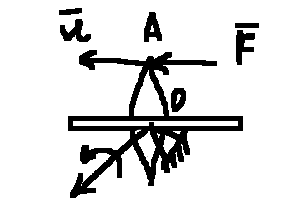
\includegraphics[scale=0.7]{img/1.png} 
    \end{figure}
    \par Допуск круглости в сечении конуса составляет 0,02 мм
    
    \begin{figure}[H]
    \centering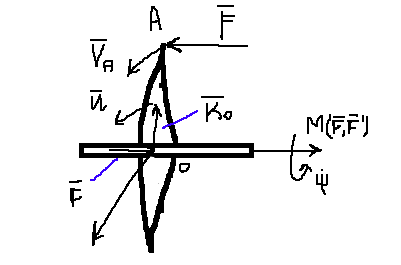
\includegraphics[scale=0.7]{img/2.png} 
    \end{figure}
    \par допуск прямолинейности образующей конуса составляет 0,01 мм
    
\end{center}
\newpage


\Large\section*{\textcolor{violet}{Лекция№3}}
\begin{center}
    \par \textbf{ВОПРОС:} можно ли проставлять допуски к нескольким поверхностям?
    \par \textbf{ОТВЕТ:} \textit{да, можно}
    
    \begin{figure}[H]
    \centering\includegraphics[scale=0.7]{img/3.png} 
    \end{figure}
    
    \par \textcolor{red}{обязательно квадрат в обозначении мм, стрелка стоит ровно по середине (ошибки можно указать на рисунке, либо написать словами, РИСУНКИ ОБЯЗАТЕЛЬНО КАРАНДАШОМ, ИНАЧЕ БУДЕТ БО-БО)}
    \par допуск к плоскостности каждой из трех поверхностей составляет 0,01мм
    \par ГОСТ3.1109-82 (все определения тащим из этого госта)
    \par Технологическая база - сочетание поверхностей, ось или точка предмета труда, используемые для нахождения положения в процессе изготовления

    \begin{figure}[H]
    \centering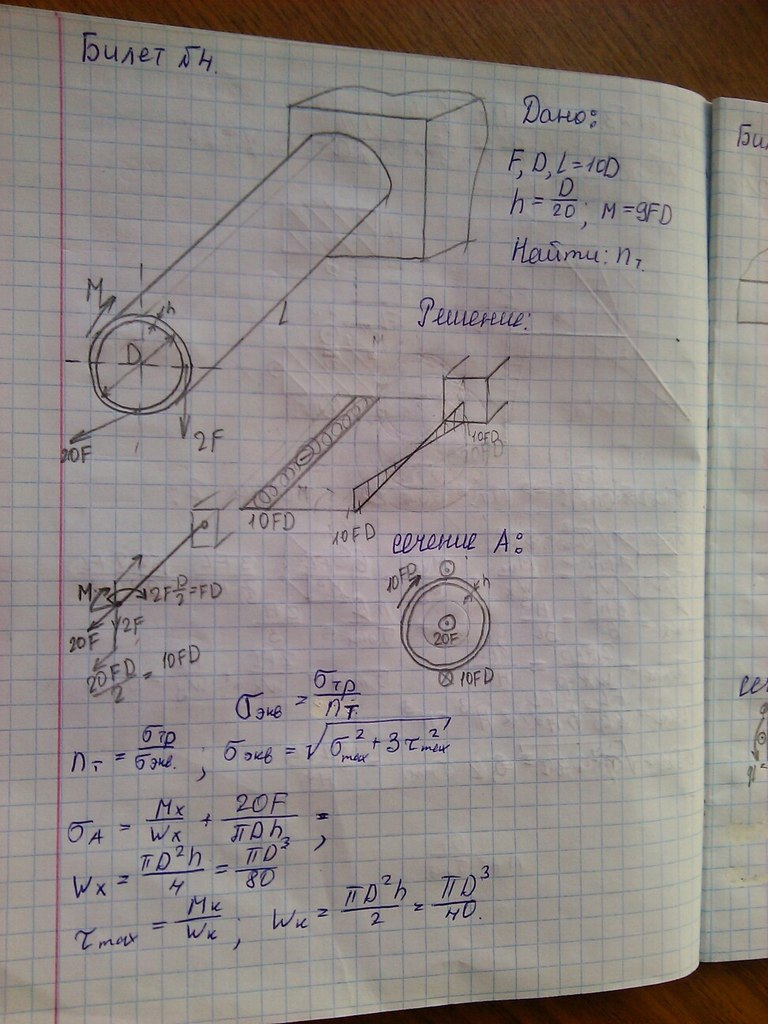
\includegraphics[scale=0.7]{img/4.png} 
    \end{figure}

    \par Допуск параллельности для каждой поверхности составляет 0,01мм
    \par (треугольник должен быть равносторонний, закрашенный, буквы обязательно в алфавитном порядке. технологическая база - квадратик, прямоугольник, квадратик)

    \par физико-механическая и геометрическая состояние поверхностей, от который зависят функциональные свойства деталей

    \par пример функциональных свойств: электро и техно проводность, корозионно и износо стойкость, прочность и контактная жесткость

    \par разница свойств слоя у поверхности и в объеме 

    \par \textbf{ВОПРОС:} всегда ли существует эта разница?

    \par \textbf{ОТВЕТ:} \textit{да, она существует, так как всегда будет происходить термическая обработка -> происходит упрочнение}

    \par макро неровность - едничное отклонение от номинальной формы детали

    \begin{figure}[H]
    \centering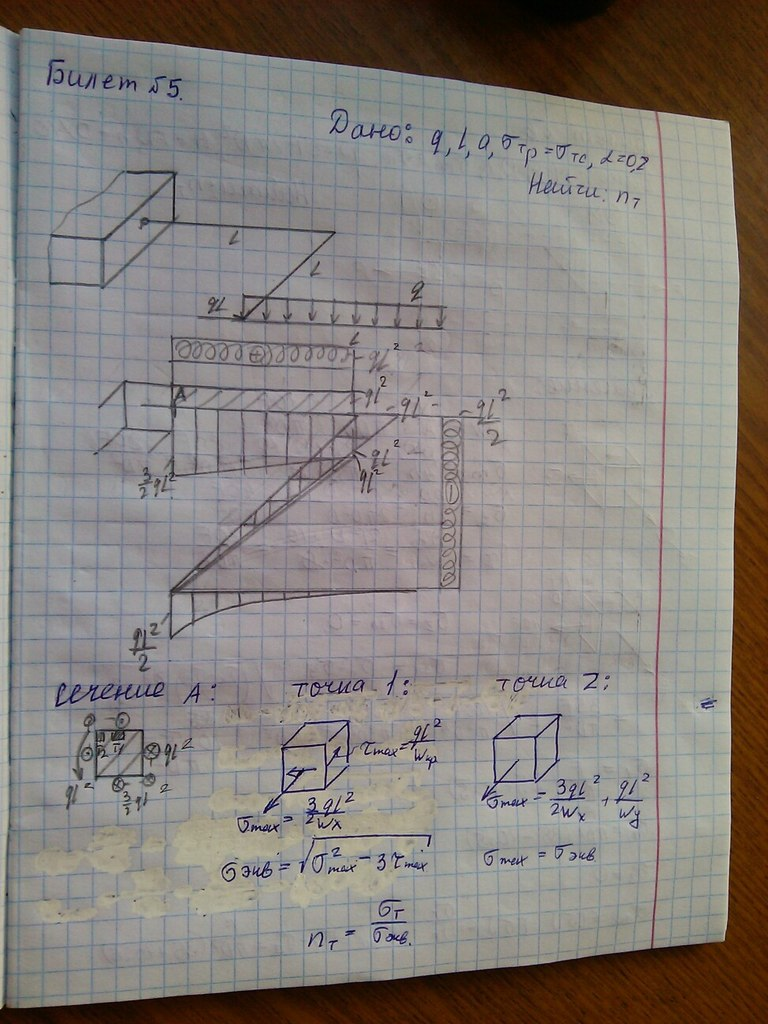
\includegraphics[scale=0.7]{img/5.png} 
    \end{figure}

    \par овальность 

    \begin{figure}[H]
    \centering\includegraphics[scale=0.2]{img/6.jpeg} 
    \end{figure}

    \par огранка

    \par Овальность лучше огранки

    \begin{figure}[H]
    \centering\includegraphics[scale=0.2]{img/7.jpeg} 
    \end{figure}
    
    \par если пошло что-то не так, то появлется макро-неровность(цилиндричность, изогнутость, карсетность, бочкообразность)

    \par бочкообразность хуже всего, так как кристаллическая решетка раздута, а при ее спиле произойдет разупрочнение

    \par волнистость - периодическое чередование выступов и впадин 
    \par (она возникает из-за вибрации в процессе механической обработки)

    \par Микро-неровность - шероховатость - совокупность чередующихся неровностей с относительно малыми шагами

    %фотка с доски яхай биля
    \begin{figure}[H]
    \centering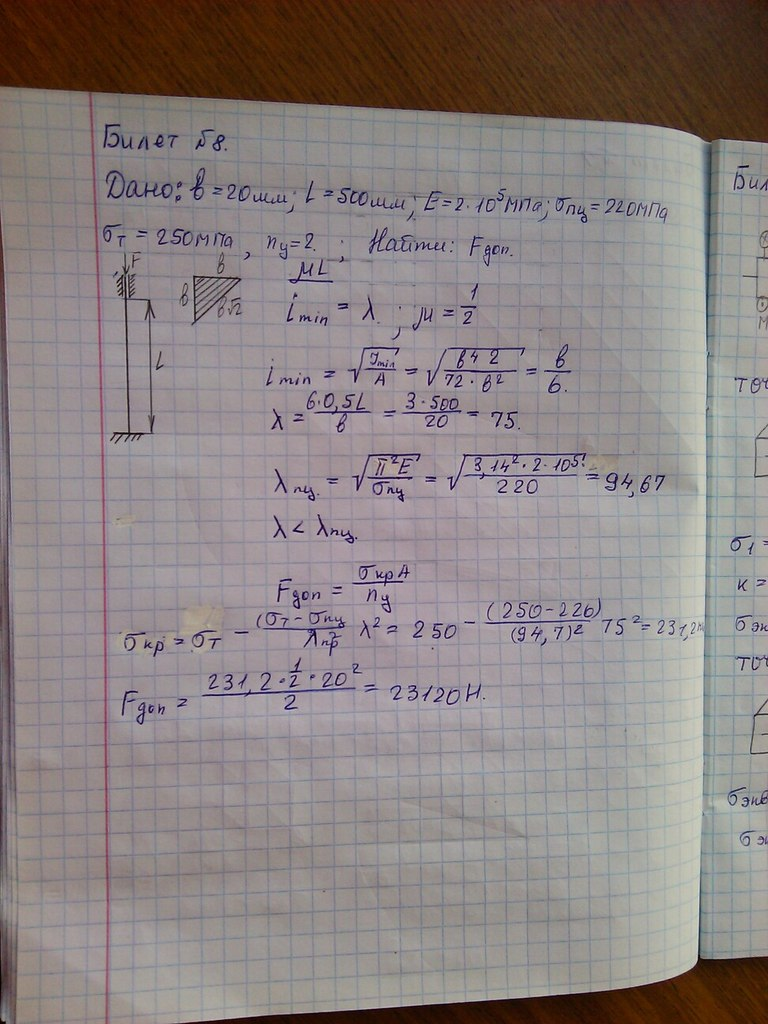
\includegraphics[scale=0.3]{img/8.jpeg} 
    \end{figure}

    \par припуск - специально предусмотренный слой материала, который удаляется механической обраткой для достижения заданых свойств.

    \par припуск всегда придусматривается, виды:

    \par 1)операционный (удаляется за одну технологическую операцию)

    \par 2)промежуточный (удаляется за один технологический переход)

    \par 50 < l/h <= 1000 - волнистая 

    \par l/h <= 50 - шероховатая

    \par направление неровностей мб параллельным, перпендикулярным, перекрещивающимся, произвольная (произвольное - самое плохое, перекрещивающиеся - норм, другие - кайф, параллельная и перпендикулярная неровность равнозначны, обе вкусные)

     %фотка с доски яхай биля 9
    \begin{figure}[H]
    \centering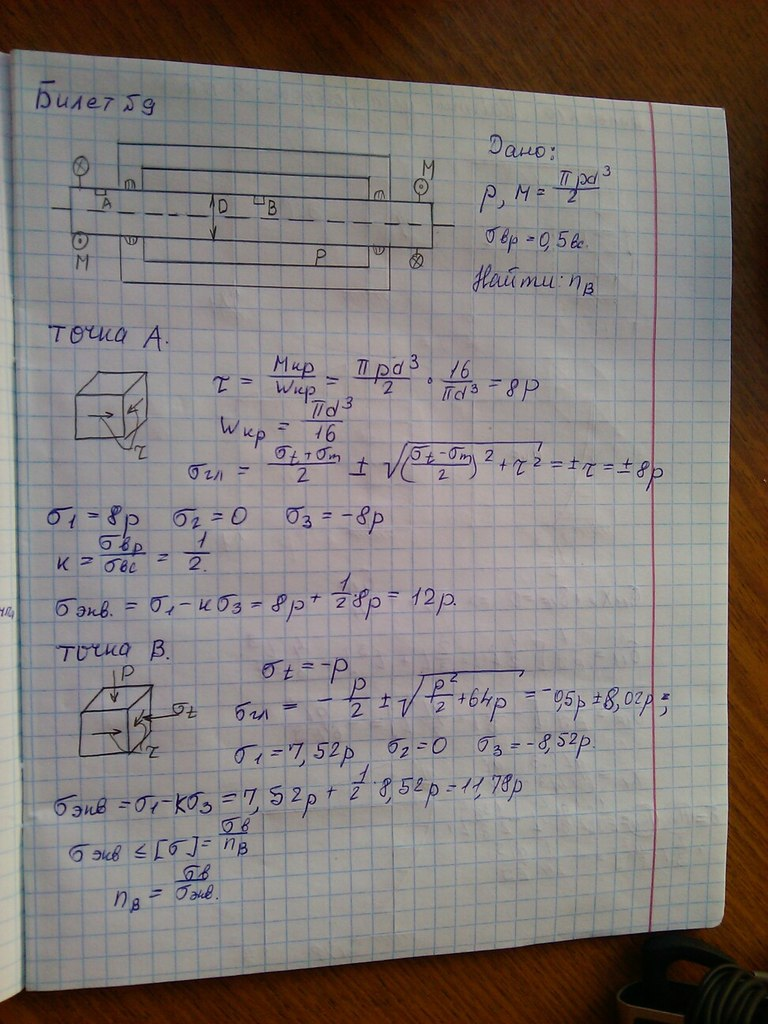
\includegraphics[scale=0.2]{img/9.jpeg} 
    \end{figure}

    ГОСТ: 2789-73, 2.309-73

     %фотка с доски яхай биля 10
    \begin{figure}[H]
    \centering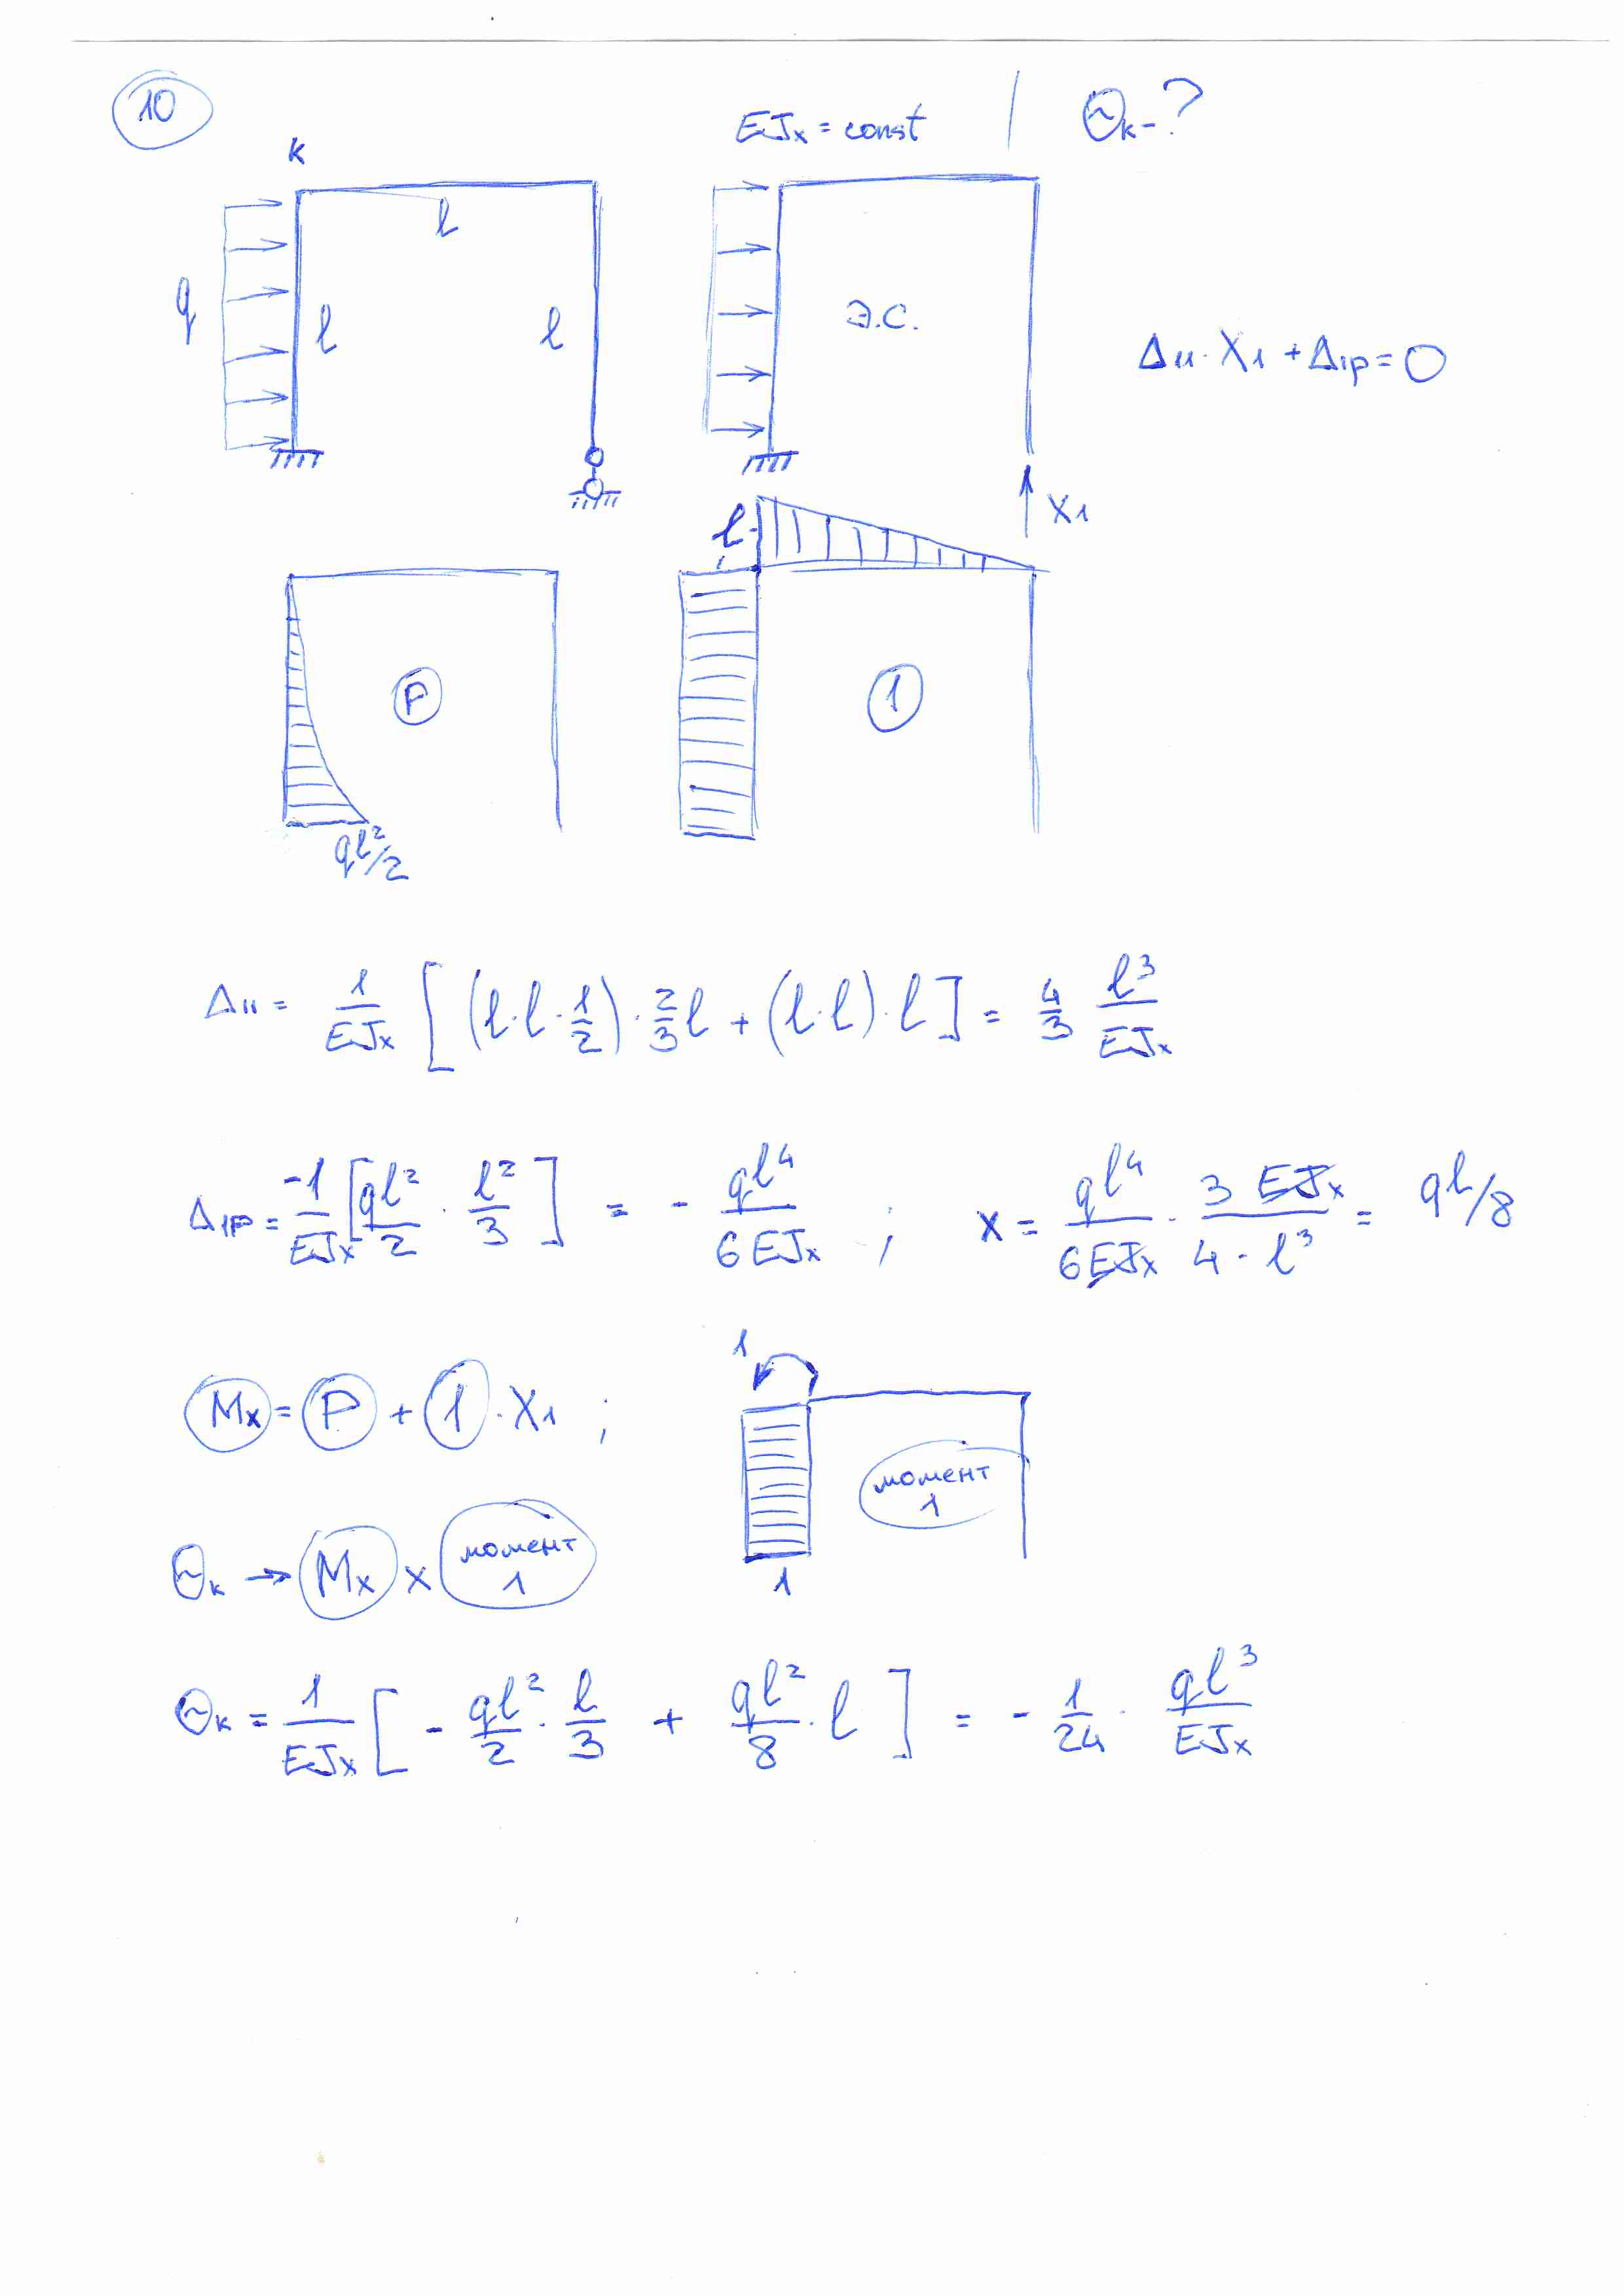
\includegraphics[scale=0.2]{img/10.jpeg} 
    \end{figure}

    \par 2)поверхность должна быть образована удалением слоя материала
    \par 3)галочка с кружочком - поверхность должна быть получена без удаления слоя материала (прям атас, почти Анастас)
    
    \par \textbf{группы методов контроля:}
    \par 1)бесконтактный, основаны на оптическом принципе, оценке интерференции, отраженных от поверхностей световых лучей и реализуются на микроинтерферометре 
    \par 2)контактный - ощупывание участка поверхности острым концом алмазной иглы и реализуются на профилографе, профилометр (профилограф лучше, сам все записывает за нас, не нужно наблюдать за ним)

    \par \textbf{Понятие о технологичности конструкции}

    \par Технологичность - совокупность свойств для оптимальных затрат при изготовлении, обслуживаний и ремонте при заданных показателях качества, объеме выпуска и условиях выполнения работ

    \par \textbf{Виды технологичности:}

    \par 1)производственная - при подготовке к производству, а также при узготовлении и монтаже вне предприятия

    \par 2)эксплуатуционная - при подготовке к использованию, обслуживанию и текущем ремонте (текущий ремонт не является обязательным)

    \par 3)ремонтный - при всех видов ремонта, кроме текущих (текущий ремонт входит в эксплуатуационный)

    \par Показатели технологичности (раздаточный материал)


    \par Купил кореец колбасу и бросил ее в холодильник к хуям собачьим.

    \par (для рк 2)

    \par Методы формообразования заготовок деталей

    \par Формообразование - это изготовление заготовки или изделия из жидких, порошковых или волоконных материалов.

    \par \textbf{Группы методов:}

    \par 1) заготовительная операция - предвариательная обработка 

    \par 2) черновая обработка (?еще название?), в результате которой снимается основная часть припуска

    \par 3) чистовая обработка (финишная обработка), в результате которой достигаются заданные точность размеров и качетсво поверхностей 

    \par привести пример обработки

    \par заготовительной : литье, обработка давлением, ?фармолание?

    \par черновая : точение, фрезирование, сверление

    \par чистовая : шлифование, полирование, притирка

    \par \textbf{Получение заготовок литьем}

    \par Получаются ли ... литьем (ответ нет)

    \par Литье - это изготовление отливки из жидкого материала путем заполнения им полости заданных форм и размеров с последо=ующим затвердиванием. 

    \par Отливка - заготовка получаемая литьем 

    \par независимо от того, какой метод литья - она называется отливкой

    \par \textbf{Классификация методов литья}

    \par от чего зависит качество отливки ?

    \par ответ: Зависит от материаа литейной формы и точности ее изготовления 

    \par Что такое литейная форма?

    \par Ответ:основной \textbf{инстурмент} при литье, придающий отливке очертание будущей детали

    \par \textbf{виды литейных форм:}

    \par 1) разовая - форма разрушается при извлечении отливки ( Пример: песчанная, песчанно-глинистая) 

    \par 2) полупостоянная - выдерживает более одной отливки. Металло керамич форма выдерживае 50-100 отливок. Графитовая - до 300 отливок.

    \par 3) постоянная - выдерживает несколько тысяч отливок ( металлическая - до 10 000 отливок) 

    \par В приборостроении используется только 1 и 3 вид (разовая и постоянная)

    \par ТАБЛИЧКА!!!!!! (Саня просто решил написать про табличку)

    \par \textbf{Требования к литейным сплавам}

    \par Сплав лучше чистого металла

    \par Сплавы делятся 

    \par 1) литые стали. Заточено именно под литье, прошло доп термообработку. Содержащие до 2 процентов (включительно) углерода

    \par разновидности стали:

    \par 1.1) углеродистые (нелегированные). характеристики - хорошая обрабатываемость резанием, но пониженные механичекие свойства. 

    \par Марка: (ГОСТ 977-88)   15Л - 0,15 процентов углерода, Л - литейная марка

    \par 1.2) низколегированные ( ГОСТ 7832 - 65 ) - содержит до 1 процента добавок. Характеризуется повышенной износостойкотью и высоким асортиментом 

    \par Марка, которая ... наивысокую износостойкость (ответ: 35 ХГСЛ)

    \par расшифруйте "35ХГСЛ".    (ответ: 0,35 углерода, Х - до 1 процента хрома, Г - до 1 процента марганца, С - до 1 процента кремния, Л - литейная марка)  

    \par расшифруйте "12ДХН1МФЛ" (ответ: 0,12 процента углерода, Д - до 1 процента меди, Х - до 1 процента хрома, Н1 -  процента никеля, М - до 1 процента молебдена, Ф - до 1 процента ванадия, Л - литейная марка) 
    
    \par 1.3) высоколегированные стали. Содержат боолее 1 процента добавок. Свойства: характеризуется обширным диапащоном рабочих температур. Привести пример стали : Х5МЛ. Она выдерживает диапазон температур -40..550C 

    \par Расшифруйте "Х88ВЛ" (Ответ: Х8 - 8 процентов хрома, В - до 1 процента вольфрама, Л - литейная марка)

    \par "Х18Н12М3ТЛ (ответ: Х18 - 18 процентов хрома, Н12 - 12 процентов никеля, М3 - 3 процента молебдена, Т - до 1 процента титана, Л - литейная марка)

    \par Содержится ли в этой марке углерод (ответ: содержится до 2 процентов)

   \par Шакал легирования: (тут должна быть картинка)
 
     %фотка с доски яхай биля 11
    \begin{figure}[H]
    \centering\includegraphics[scale=0.2]{img/11.jpeg} 
    \end{figure}

    \par 2) Чугуны (содержит более 2 процентов углерода)

    \par 2.1) белые чугуны. свойсвта: характеризуются повышенной корозионной износостойкостью а также жаропрочностью

    \par почему чугуны характеризуются? ответ: они выдерживают до 1000 град цельсия 

    \par Расшифруйте "Х34Л" (ГОСТ 2176 - 77) (для чугунов) (Ответ: Х34 - 34 процента хрома, Л - литейная марка, до 2,2 процента чугуна.)

    \par 2.2) Высокопрочне. характеризуются повышенной прочностью, пластичностью и вязкостью.

    \par Расшифруйте "ВЧ60-2" (ответ: В - высокопрочный, Ч - чугун, 60 - предел прочности при растяжении = 60 кг * с / $\text{мм}^2$ = 588 Н/$\text{мм}^2$, тире - разделительный знак, 2 - относительное удлинение (сигма) = 2 процента) 

    \par 3) Аллюминиевые сплавы (характеристики - характеризуется низким удельным весом, высокой тепло и электро проводностью, прочностью, хорощая обрабатываемость резанием)

    \par Расшифруйте "АЛ1" (ответ: А - алюминиевый сплав, Л - литейная марка, 1 - ???) 

    \par наилучшие литейные свойства (в порядкке убывания): АЛ2 , АЛ4, АЛ5, АЛ9, АЛ13, АЛ26, АЛ30.

    \par 4) Магниевые сплавы. Характеризуется самым низким удельным весом, пониженной тепло и электро проводностью, высоким уровнем демфирвоания и хрупкостью при высокой темперауре.  

    \par Демфирование - способность гасить вибрации.

    \par почему примениение магния нежелательно в приборостроении?  ответ : обращования оксида магния сопроводлается выделением большим кол-вом энергии, что может привести к самовоспламененю или даже взрыву 

    \par Расшифруйте "МЛ2" (ответ: М - магний, Л - литейная марка, 2 - модификаци)

    \par Какие марки наибольшей литейной свойствами (МЛ5, МЛ6)

    \par 5) Медные сплавы. 

    \par 5.1) литейные латуни (спав меди с цинком). характеризуется высокой коррозионной стойкостью и хорошими механич свойствами. 

    \par Расшифруйте "ЛК80-3Л) (ответ: Л - латунь, К - добавка кремний, 80 - 80 процентов меди, тире - разделительный знак, 30 - 30 процентов (добавки) кремния, Л - литейная марка, цинка 17 процентов (рассчитывается как остаток от вычитания))

    \par Расшифруйте "ЛС59-1Л" (ответ: Л -латунь, С - свинец, 59 - 59 процентов меди, тире - разделительный знак, 1 - 1 процент (добавки) свинца, Л - литейная марка)

    \par \textbf{Лекция 13.03}

    \par литые оловянные бронзы 

    \par Расшифруйте "БрОЦС4-4-2,5Л" (ответ: Бр - Бронза, О - основная добавка Олово, Ц - добавка цинка 4 проц, С - добавка свинца, 4 - проц содержание олова, - - разделительный знак, 4 - проц содержание цинка, - - разделительный знак, 2,5 - проц содержание свинца, Л - литейная марка )

    \par Бронза характеризуется высокой коррозионной стойкостьью и хорошими литейными свойствами

    \par Литые безоловянные бронзы (альтернативное название: специальные бронзы)

    \par Расшифруйте "БрАЖН10-4-4Л" (ответ: Бр - бронза, А - аллюминий, Ж - железо, Н - никель, 10 - проц содержание Алюм, - - разделит знак, 4 - проц содержание 

    \par характеризуются высокой тепло и электропроводностью и хорошими механическими свойствами

    \par общее свойства медных сплавов - дороговизна.

    \par Цинковые сплавы

    \par Расшифруйте "ЦАМ4-3" (ответ: ц - цинк, А - алюм, М - медь, 4 - проц содерж алюм, - - разделит знак, 3 - проц содержание меди)

    \par характеризуются высокой прочностью но большой подверженностью старения

    \par недостаток: большая подверженность старения 

    \par Титановые сплавы

    \par какая область применения титана - идут на простые детали приборов, работающих до темп 450 град цельсия. 

    \par расшифруйте "ВТ6" (ответ: В - высокопрочный, Т - титановый сплав, 6 - модификация)

    \par чем характер - характеризуется низкой тепло и электропроводностью, высокой корозионной стойкостью, прочностью, но дороговизной . По удельной жаропрочностипревосходит алюмин и магниеые сплавы и даже легированные стали

    \par попоулярность записывалась в порядке убывания популярности! (титан самый непопулярный)

    \par можно ли избавиться от усадки (ответ: нет) усадка есть всегда

    \par что происходит после охлаждения отливки и извлечения ее из формы? (ответ: после охлаждения отливки и извлечения ее из формы есть еще 2 этапа: 1) очистка поверхностей готовой отливки 2) термообработка) 

    \par являются ли эти этапы обязательными? (ответ: очистка - необязательна, термообработка - обяззательна)

    \par для чего служит термообработка? (ответ: для улучшения структурф отливки, повышения обрабатываемости резанием, и снятия остаточных напряжений)

    \par какой недостаток остаточных напряжений? (ответ: приводит к короблине)

    \par приведите пример термообратоки приборостроения?? (ответ: 4 вида: 1) закалка  2) нормализация 3) отжиг 4) отпуск)

    \par приведите 3 примера (выкидываем какое-то одно см. выше)
    
    \par применяется ли оБжиг в приборостроении? (ответ: нет)

    \par \textbf{литье в разовые формы: (три следующие)}

    \par литье в землю (альтернативное название - литье в песчанные формы)

    \par литье в оболочковые формы 

    \par литье по выплавляемым моделям

    \par \textbf{литье в постоянные формы:} 

    \par литье в кокиль

    \par литье под давлением 

    \par центробежное литье

    \par какие методы литья применяются в приборостроении? (ответ: литье по выплавляемым моделям, литье в кокиль, литье под давлением)

    \par т\textbf{ехнологические требования к конструкциям отливок}

    \par 1) равностенность

    \par для чего нужна равностенность? (ответ: чтобы избежать усадочных раковин из-за неравномерности усадки)

    \par ребра жесткости рассчитываются по слежующей формуле:

    \par $S_{реб}$ = (0,8 .. 0,9) Sср  (Sср - средняя толщина стенки) на рк выбираем 0,9!!!!

    \par 2) тонкостенность 

    \par зачем нужна тонкостеность (ответ: чтобы избежать крупносзернистой структуры отливки)

    \par 3) скругления

    \par допустимы ли острые углы при отливке??? (ответ: да, но лишь на плоскотсях разъема формы, а в остальных местах сопряжения стенок должны быть радиусы скругления)

    \par ФОТО ВСТАВЛЯЙ БИЛЯ СКРУГЛЕНИЯ МАНА
    %фотка с доски яхай биля 4
    \begin{figure}[H]
    \centering\includegraphics[scale=0.8]{img/12.png} 
    \end{figure}

    \par еслм ллитье в землю , то К = от 3 до 4,  если в "???" - то от 4 до 5, если по выплавляемым моделям - то от 3 до 5, если литье в кокиль - то от 4 до 6, если литье под давленим - то от 8 до 12

    \par радиусы внутреннего сопряжения округлить до ближайшего бОльшего числа соответсвующего радиусу стандартной фрезы

    \par ряд радиусов стандартных фрез : 1, 2, 3, 5, 8, 15, 20, 25, 30, 40 мм  (только такие радиусы внутреннего сопряжения) 

    \par радиусы внешн - не надо округлять

    \par плавные переходы

    \par почему нужны плавные переходы? (ответ: чтобы избежать образования трещин из-зи неравномерной кристаллизации)

    \par ФОТО ПЛАВНЫХ ПЕРЕХОДОВ ВСТАВЛЯЙ БИЛЯ
    %фотка с доски яхай биля 4
    \begin{figure}[H]
    \centering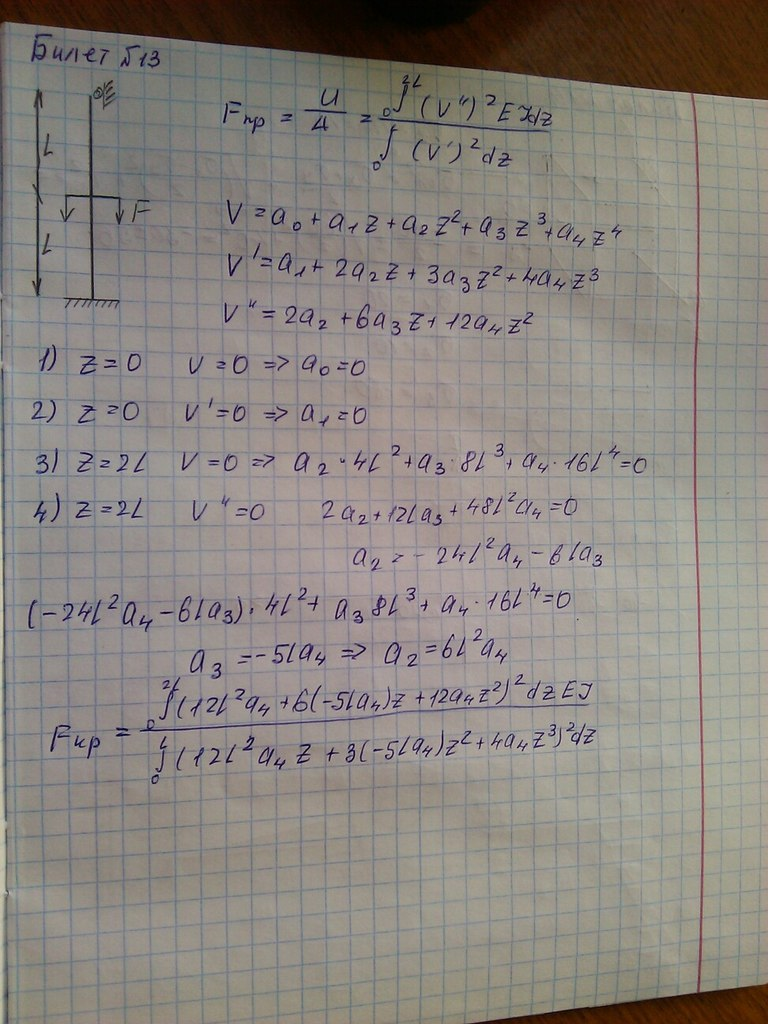
\includegraphics[scale=0.8]{img/13.png} 
    \end{figure}

    \par что являтеся технологичных и что явдяется оптимальным 

    \par 1) нетехнологичный --> не оптимальный (заготовка пределывается)

    \par 2) технологичный --> неоптимальный (нерекомендуется так делать)

    \par 3) технологичный --> оптимальный

    \par Полости и отверстия

    \par рекомендуются получать литьем а не послежующей мех обработкой, чтобы избежать скрытия в утолщенных частях отливки воздушных газовых и усадочных раковин а также появления пузырей.

    \par глубокое отверстие - то отверстие, в котором следующее (l > 3d) l - глубина отверстия d - диаметр

    \par с обеих сторон отливают глухие отверстия с перемычкой, которая затем удалятся мех обработкой 

    \par ФОТО глубоко отверстия с перемычками БИЛЯ
    %фотка с доски яхай биля 4
    \begin{figure}[H]
    \centering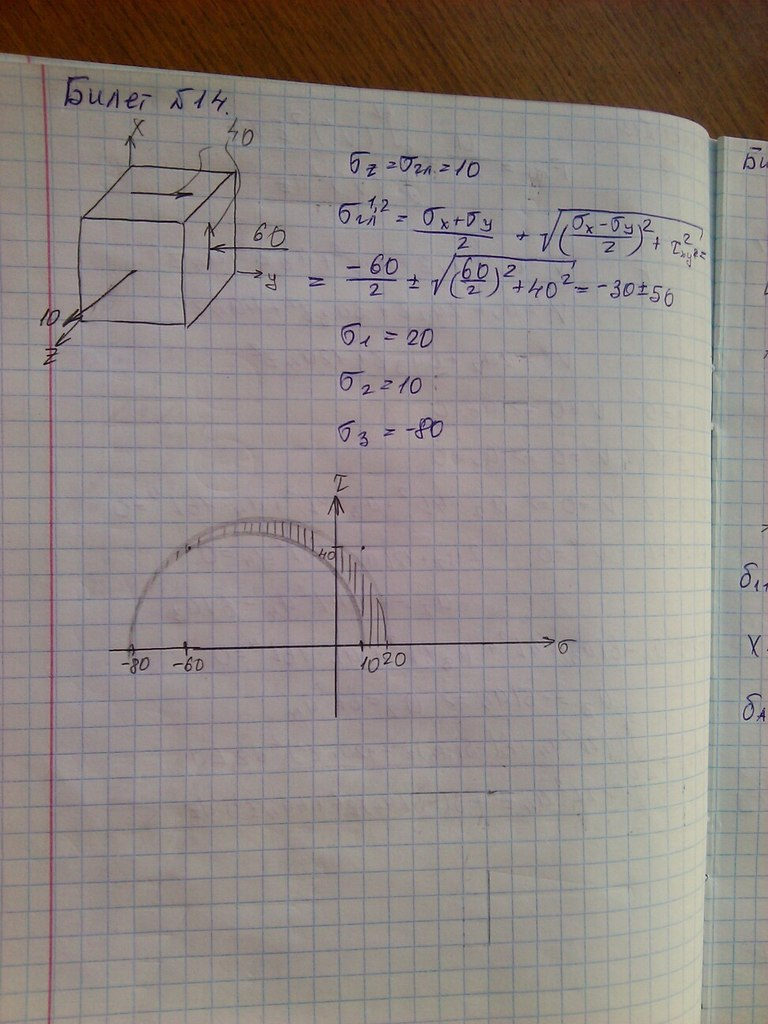
\includegraphics[scale=0.8]{img/14.png} 
    \end{figure}

    \par \textbf{Армирование}

    \par - это усиления частей конструкции элементами из другого более прочного материала 

    \par для чего служит армирование (ответ: для исключения сборочных операций, для обеспечения равностенности)

    \par такая заготовка перестает быть деталью (ПО ОПРЕДЕЛЕНИЮ) становится сборочной единицей
\end{center}
\newpage

\Large\section*{\textcolor{violet}{Лекция№4}}
\begin{center}

    \par \textbf{Обработка давлением}

    \par очень популярна - в приборостроении получают до 80 проц всех заготовок именно жтим методом

    \par Обработка давлением - пластическое деформирование или разделение материалов без образования стружки под действием давления, превышающего силу сцепления молекул 

    \par интрументы: кролик, шарик со свободной осью вращения и боёк-чекан

    \par рабочее тело: шарик из стали, стекла или пластмассы и дробь

    \par классификация способов обработки давлением, их особенности...

    \par I) бесштамповые  

    \par штамп - это оснастка, посредством которой заготовка преобретает размеры и формы соответсвующие поверхности или контуру рабочих элементов штампа 

    \par узлы и детали штампа: рабочий элемент, блок, клин, ползушка, пакет, хвостовик, обойма, трафарет, отлипатель

    \par II) бесштамповые

    \par 1) прокатка (холодная обработка предпочтительнее, так как не надо греть (дешевле))    --  горячая обработка 

    \par литая болванка многократно уплотняется путем обжима между вращающимися валками прокатного стана чтобы повысить прочность и герметичность заготовки из прокатки

    \par виды прокатки: сордовой (предпочтительный) и несордовой ???(хер знает - не успел записать) 

    \par сордовой - квадратные, листовые (тоже прослушал)

    \par примеры заготовок (валы, втулки, стаканы, крепежные детали, рычаги, фланцы, кольца) 
    
    \par КАРТИНКУ ВСТАВЛЯЙ БИЛЯ1

    \par угол захвата заготовки валками

    \par условие захвата - $K_{Tp} >= tg \alpha$

    \par от чего зависит Ктр? от температуры заготовки, скорости прокатки, от щероховатости поверзности валков и их смазки

    \par виды деформации 

    \par обжатие: $\Epsilon_{h} = \frac{h_H - H_k}{h_H}$

    \par уширение (увеичение ширины): $\Epsilon_{b} = \frac{b_k - b_H}{b_H}$

    \par вытяжка (увеличение длины): $\Epsilon_{l} = \frac{l_k}{l_H}$

    \par недостатки прокатки: небольшие размеры проката, не каждый прокатный металл имеет во всех направлениях одинаковую плотность и прочность из-за шлаковых включений

    \par 2) накатка: образование резьбы, мелких рефлений и зубьев непосредственно воздействием инструмента.  (хололдная обработка)

    \par Картинка 2 БИЛЯ

    \par 3) волочение

    \par какая обработка? - холодная обработка

    \par заготовка протаскивается через сужающиеся отверстия волочильного стана и постепено вытягивается в нить или трубку

    \par Картинка 3 БИЛЯ (волочильный стан)

    \par 1) обойма 2)рбочая зона 3) каллибрующая зона 4) выходная?? зона

    \par вопрос про деформацию

    \par формула деформации: $\Epsilon = \frac{F_H - F_k}{F_H}$

    \par 4) протягивание

    \par заготовка проотаскивается  через вращающиеся ролики протяжного стана

    \par оборудование: стан

    \par прикладываемое усилие значительно меньше чем при волочении.

    \par протягиванием целесообразно получать мелкие однотипные детали из проката 

    \par  Способы с применением штампа (дороже)

    \par 1) выдавливание (горячая обработка)

    \par заготовка сжимается замкнутой полости, а ее материал вытесняется наружу через отверстие заланного диаметра

    \par КАРТИНКА 4 БИЛЯ

    \par штамп состоит из двух составных чатей (матрица и пуансон)

    \par где происходит выдавливание? (на гидравлическом прессе)

    \par какая скорость истечения металла (0.2 .. 2 м/с)

    \par $\Epsilon = \frac{F_{koHTp}}{F_{maTp}}$

    \par плозадь отверстия контейнера, площадь отверстия матрицы

    \par недостатки выдавливания: возникновение торцового заусенца между пуансоном и матрицей при $\epsilon > 7,5..8,0$ и большие отходы производства

    \par для крупных труб отходы составляют до 45 процентов

    \par 2) объемная штамповка

    \par 

    \par 

    \par 

    \par 

    \par 

    \par 

    \par 

    \par 
    
    \par 

    \par 

    \par 

    \par 

    \par 

    \par 

    \par 

    \par 

    \par 

    \par 

    \par 

    \par 

    \par 

    \par 

    \par 

    \par 

    \par 

    \par 

    \par 

    \par 

    \par 

    \par 

    \par 

    \par 

    \par 

    \par 

    \par 

    \par 

    \par 

    \par 

    \par 

    \par 

    \par 

\end{center}

\end{document}
